\documentclass[11pt]{article}

\usepackage[utf8]{inputenc}
\usepackage[english]{babel}
\usepackage[T1]{fontenc}
\usepackage{blindtext}

\usepackage{graphicx}
\usepackage{float}
\usepackage{subcaption}
\usepackage{textcomp}
\usepackage{amsmath, amssymb}
\usepackage{multicol} % For multiple columns
\usepackage{geometry} % For adjusting page margins

\usepackage[
backend=biber,
style=numeric,
sorting=ynt
]{biblatex}
\addbibresource{email-topology.bib} % Import bibliography from bib file

\pdfsuppresswarningpagegroup=1

% Set page and column margins
\geometry{margin=1in}

\setlength{\parindent}{1.5em}

\title{Replication and impact analysis of\\"Scale-free topology of e-mail networks" }
\author{Jack Margeson\thanks{Additional author information: https://marg.es/on}\\
University of Cincinnati, College of Engineering and Applied Science}
\date{\normalsize{(Dated: November 16, 2023)}}

\begin{document}

\maketitle

\vspace{-3mm} % Move abstract up towards title

\begin{abstract}
    An analysis of the paper "Scale-free topology of e-mail networks" by Holger Ebel, Lutz-Ingo Mielsch, and Stefan Bornholdt. While unable to recreate experimental results one-to-one, findings using a dataset matching the paper provided by the book "Network Science" are presented. An examination on how the paper has impacted the field of network science is performed by summarizing two papers citing the original. Included are thoughts on interesting topics of discussion further building on the work done by Ebel et al. The report concludes that the original paper has had a great impact on the field of network science as a whole and is a good example of why the field of network science should continue to be studied.   
\end{abstract}

\vspace{5mm} % Add spacing after abstract

\begin{multicols}{2}

\section{Introduction}
\hspace*{\parindent}This report serves as both a replication study and impact analysis on the text "Scale-free topology of e-mail networks" \cite{1} by Holger Ebel, Lutz-Ingo Mielsch, and Stefan Bornholdt. 

Following this introduction is a summary outlining the goals and results of the original paper. The summary leads into the replication of major findings from the paper, completed with a sanitized copy of the original dataset using NetworkX, a Python package with the purpose of creating, manipulating, and analyzing complex networks. The full source code for all replications performed can be found in a public GitHub repository \cite{2} from the author of this report. 

After the presentation of replications, an analysis is conducted on two identified examples of impactful work done by Mao et al. \cite{5} and Xie et al. \cite{4} that have been produced citing the "Scale-free topology of e-mail networks" paper. Finally, a section theorizing two interesting directions for future research in the fields of cybersecurity and social networks using e-mail network analysis is provided.

\section{Summary}
\hspace*{\parindent}In the original text, Ebel et al. study a network consisting of sent and received e-mails. The data set used for the study was obtained by observing the log files of an e-mail server located at Kiel University. The authors of this paper were able to construct a network based upon this data, in which the nodes represent individual e-mail addresses and links between them represent a delivered e-mail. Several mathematical analyses were conducted in order to deduce information that could help classify the network. 

The general conclusion found from these analyses was that their network " exhibits a scale-free link distribution and pronounced small-world behavior" \cite{1} that aligns with the findings of similar studies on various other social-based networks. Implications for these findings, including the importance of the scale-free property of the network on the spread of e-mail viruses, are touched upon briefly towards the end of the paper. 

\subsection{Strengths}
\hspace*{\parindent}The greatest strength of the original paper is undoubtedly that it established a line of reasoning to determine the degree distribution of e-mail networks to exhibit a power law, providing evidence towards e-mail networks being scale-free. Additionally, not only did the authors find evidence that e-mail networks could be considered scale-free, they also found that the e-mail network that they had created from their sample data exhibited small world behavior, which indicates that node neighbors of a node are likely to be connected themselves. These two findings have been instrumental in future e-mail related studies, two of which will be talked about in the impact analysis section of this report.	

\subsection{Weaknesses}
\hspace*{\parindent}There are a few small albeit important weakness to mention present in the original paper. Justifications for these weakness are provided via opinion of the author of this report.

One issue that arises in the fact that the sampling process is restricted to exclusively one e-mail server. However, it would generally be unreasonable for the authors of the paper to acquire data from other universities or similar group-based entities with an emphasis on e-mail communication. This is due to the fact that a data set of e-mails as large as the one presented in the original paper would have to be extensively cleaned as to not expose sensitive data, which would take time and energy on the part of the group providing the dataset. Given this information, it is unlikely that another dataset to enforce preliminary findings would not be feasible to obtain for the original paper authors, leaving the task of replication with alternate datasets to other publications.

While not directly an issue with the paper itself, an problem arises with the dataset commonly distributed for this paper. As part of this replication research, a copy of the dataset used in the original paper was taken from the "Network Datasets" section of the site hosting the "Network Science" book by Albert-László Barabási \cite{3}. However, this dataset is mildly incomplete when comparing some of the provided data to the stated statistics in the paper. For starters, a quick NetworkX network reconstruction and analysis of the graph shows us that there are a total of \(N = 57,	194\) nodes provided, while in the paper, it is stated that a total of \(N = 59,912\) nodes exist overall, with a subset of \(N = 56,969\) nodes making up a giant component in the network. Other inconsistencies, such as the lack of labels when it comes to which nodes are considered student e-mail nodes, has made it difficult to accurately replicate findings, which will be touched upon for each of the replications presented in this report. 

\section{Reproduction}
\hspace*{\parindent}As stated in the weaknesses section of this report, the distributed dataset has a few small problems when it comes to making a one-to-one replication of the original study. Below are the findings from the replication study. In cases where values or figures differ from the original paper, a justification is provided for why the discrepancy might have occurred. Findings that are unreproducable given the dataset are also discussed. 

\subsection{Network analysis}
\hspace*{\parindent}There are a few examples of network analysis that do not tie directly into a figure from the original paper. This section talks about these from a mathematical standpoint, without the use of figures. The first, which was mentioned previously, is the size of the network. Given the edgelist, we are able to reconstruct the graph structure through NetworkX to see that a total of \(N = 57,194\) nodes exist in the graph. The paper states in a footnote that three email addresses have been excluded as artifacts, due to the fact that they represented such a large degree as to be designated an outlier. By sorting our list of nodes by degree, we are able to query the last five, resulting in the following list:
\begin{align*}
[('13498', 802), ('11798', 1020), ('13678', 1228), \\('11028', 4171), ('32199', 6553)]
\end{align*}

We see that the last five nodes here have a degree greater than \(800\). Putting that in context of our e-mail scenario, these nodes are e-mail addresses that have connected to at least eight hundred other e-mail addresses (either receiving or sending an e-mail). This can be most likely explained by email servers, such as the university sending emails out to large subsets of students, as explained in the original paper. Another potential explanation for seeing these addresses with such large degrees could be in the inclusion of addresses that participate in advertisement or spam. In order to reduce the impact that these nodes have on our distributions, we will remove them from any future calculations unless otherwise stated.

After the removal of the outlier nodes described, we sum the degrees of all nodes and divide by \(N = 57,189\) to receive a mean degree of \(\langle k \rangle=3.01\), which is close to the mean degree of nodes of the giant component listed in the original study, \(\langle k_{large} \rangle = 2.96\). While not exact, a variance of \(\langle k \rangle \pm 0.05\)  between the original and calculated mean degree can be written off as negligible. 

As discussed in the weaknesses portion of the summary, the problem with the dataset is that it is completely stripped of all labels. This means for replication steps that require student-only nodes, we will have to approximate a subnetwork that can serve for our replication purposes. The second graph presented in the original paper outlines the student account degree distribution, where only nodes that represent student e-mail addresses are contained. An approximation of this student-only dataset can be created by limiting the max degree that we consider "student-owned" over the network. In essence, we want to find a subset of nodes in the network that we can justify as belonging to a student in terms of the number of other e-mail addresses that they are in association with. 

We will define \(k_{upper}\) to represent the maximum degree that we are willing to include in our student-only node network. To find a reasonable value for \(k_{upper}\), we can take a look at the mean degree of just the student nodes, identified in the paper as \(\langle k \rangle =2.88\). Using this mean degree and a sorted list of nodes by their degree, we can remove \(N\) nodes from the distribution until we get a mean degree approximating \(\langle k \rangle =2.88\):
\begin{align}
\langle k \rangle \approx 2.88 = \frac{1}{N^{'}} \sum_{i=1}^{N^{'}} k_i \\
\intertext{where $N'$ is the first node in the sorted list with degree $k_{\text{upper}}$.}\notag 
\end{align} 
\hspace*{\parindent}Using NetworkX, we find that removing the highest 27 entries from the dataset (22 additional nodes removed than the 5 outliers removed previously), we find an average degree \(\langle k \rangle = 2.8793 \approx 2.88\), giving us \(k_{upper} = 266\). Putting this number in context, it means that the maximum number of e-mail addresses that we'd reasonably expect a student e-mail address to be connected to is 266. 

We make the assumption that any of the nodes we've just removed were result of either smaller university owned e-mail accounts or students that receive an unusual amount of mail (teaching assistants, perhaps). Again, the reason that we must speculate the number of student nodes here is due to the fact that the dataset provided contains no labels on if an e-mail address node belongs to a student or not. The subset of nodes with degree equal to or less than 266 that we have just created will be used for calculating student e-mail account exclusive statistics and degree distributions.

\subsection{Degree distribution}
\hspace*{\parindent}The first degree distribution, shown in the first graph \cite{1}, encompasses all nodes in the graph minus the outliers. In the network analysis section, we removed outliers from our supplied data set. While the exact parameters for graphing were not provided, we can assume that a bin size greater than one is used due to the fact that there is a limited number of points on the plot far less than the actual number of total nodes. Graphing this revised distribution on a double logarithmic scale with a bin size of 100 gives us a figure with similar features to that of the original. A comparison between the two is presented in Figure 1.

\begin{figure}[H]
  \centering
  \begin{subfigure}{0.9\linewidth}
    \centering
    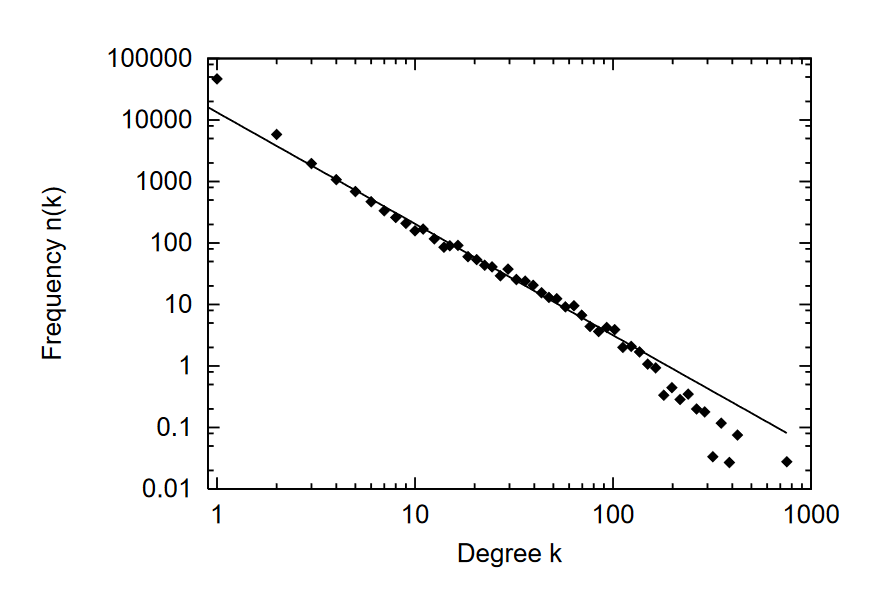
\includegraphics[width=\linewidth]{figure1_original.png}
    \label{fig:figure2_original}
  \end{subfigure}
  \begin{subfigure}{0.8\linewidth}
    \centering
    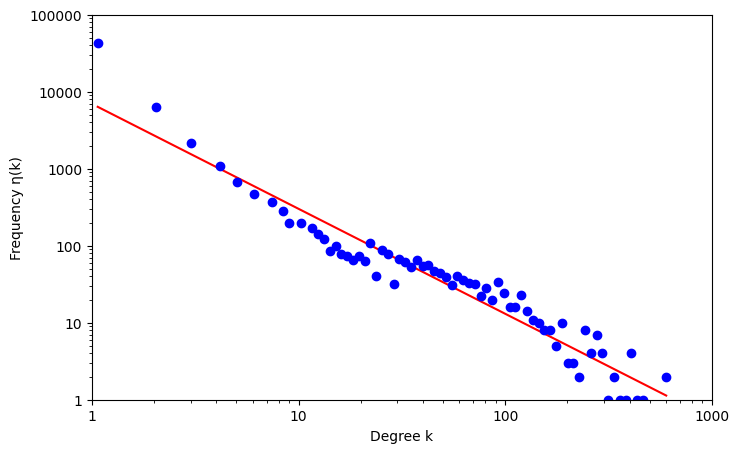
\includegraphics[width=\linewidth]{figure1_replicated.png}
    \label{fig:figure2_replicated}
    \footnotesize{Figure 1: Original figure from paper (top) and replication (bottom).}
  \end{subfigure}
\end{figure}

The final replication of the standard dataset degree distribution is similar to the findings presented in the original paper in many ways. Since both are graphed double logarithmically, a negative linear trend can be observed. Around degree values 80 to 60, there seems to be a clump of values close together that heavily impact the direction of the best-fit line. This indicates that a majority of the people owning e-mail addresses are connected to around 60-80 other email addresses. 

One observed difference between the two distributions is the scale presented on the y-axis. While many different configurations of Matplotlib (the Python package used to construct the visual graphs) were tried, such as manually plotting log-by-log graphs and normalizing the bins, a scale displaying values below 1 for the frequency was unable to be achieved. While disappointing that the original y-scale of the graph could not be represented here, we are still able to see that the recreated distribution strongly correlates with the original distribution due to the spread and location of bins that are plotted.

\subsection{Student account degree distribution}
\hspace*{\parindent}In the original paper, all student nodes are separated from the network and analyzed as to create a network that was free from external influence (such as advertisement e-mails or spam e-mails). Since the dataset provided from the "Network Science" book is unlabeled (a problem discussed earlier), the replicated distribution will rely on the network that we theorized upon during network analysis. A comparison between the two figures is presented in Figure 2.

\begin{figure}[H]
  \centering
  \begin{subfigure}{0.9\linewidth}
    \centering
    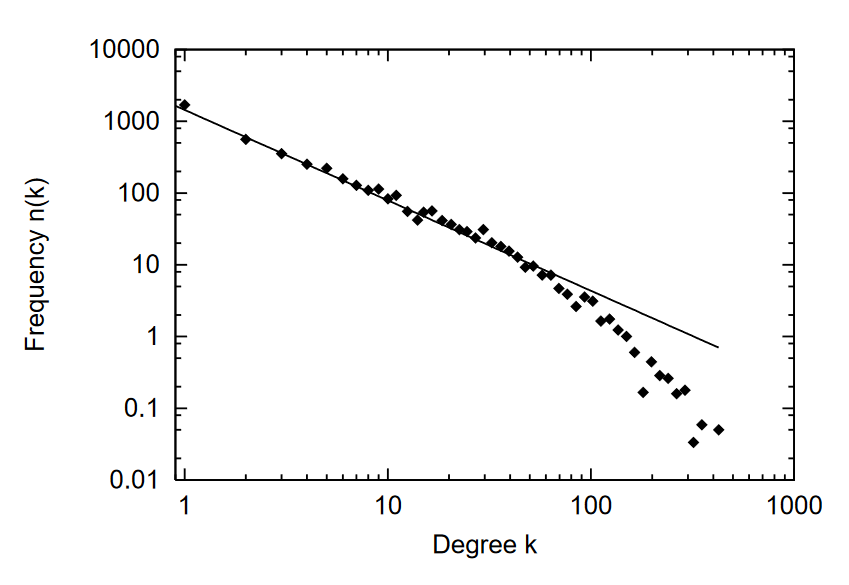
\includegraphics[width=\linewidth]{figure2_original.png}
    \label{fig:figure2_original}
  \end{subfigure}
  \begin{subfigure}{0.8\linewidth}
    \centering
    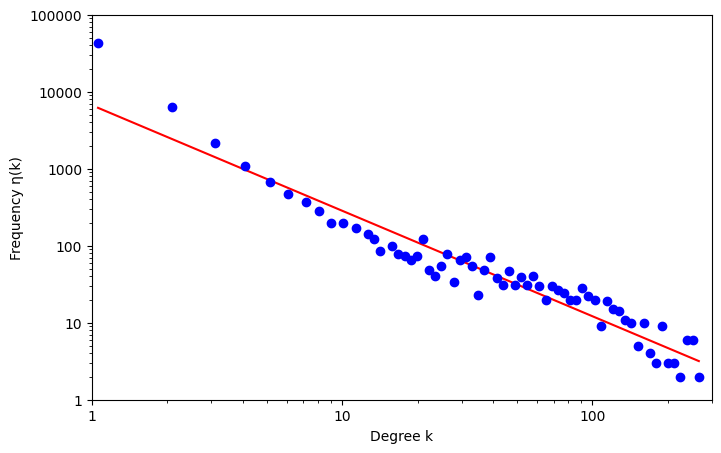
\includegraphics[width=\linewidth]{figure2_replicated.png}
    \label{fig:figure2_replicated}
    \footnotesize{Figure 2: Original figure from paper (top) and replication (bottom).}
  \end{subfigure}
\end{figure}

The original distribution for the student subset network and the replicated distribution shown have some similarities and differences. In the same fashion as the first original plot, a binning function was used to collect data points in a certain range to make the graph clearer. Here, for the replication of the student network, an estimated bin size of 100 was used. A negative linear trend (given that the plot is double logarithmic) can be again observed in both figures, with degrees maxing out in the 200-300 range. This is to be expected with our calculated \(k_{upper}=266\), which has served well in lieu of a complete labeled dataset.

The major difference between the original and the replication of the student-only network comes in the form of the right tail. In the original graph, the right tail of the distribution sags lower in frequency in degrees higher than 100. This increased negative trend is not well visible on the attempted replication figure, which could be due to several reasons. One potential reason could be that the issue from the first replication appears again, in which the y-scale is not able to accurately represent degree values greater than zero but less than one due to limitations in Matplotlib software. Another explanation might be that the size or method of the binning function differs slightly from the original paper, which could explain different visual representation for where points are being plotted on the figure. Nevertheless, the replication does display a majority of the main features displayed in the original figure.


\subsection{In/Out-degree distribution}
\hspace*{\parindent}The final two figures presented in the original paper displayed the degree distributions for exclusively the in-degree and the out-degree of the nodes for the network. Due to the fact that the dataset provided is unlabeled, we are unable to replicate any findings that relate to in-degrees or out-degrees. However, the original paper does bring up a few interesting points as it relates to the separation of in/out-degrees in this manner. It is stated that the in the context of virus spreading, which is touched upon at the end of the original paper, the graph must be treated as undirected due to the fact that the propagation of computer worms is undirected. One of the biggest areas of study that relates to the social aspect of e-mail networks is cybersecurity. Given that the goal of most viruses and cyber attacks is to spread as far as possible, it is unlikely that the research done into an in/out-degree distribution is of much substance to the cybersecurity research community. 

On the other hand, it is important to note that the original paper makes a very good case for why in-out degree analysis might be useful: "it seems reasonable that the sending and receiving of e-mails are governed by different processes" \cite{1}. Studies that utilize mechanics that apply specifically to one action, either the sending of receiving of e-mails, would be a good use case for an in/out-degree analysis. While a replication was unable to be performed in this section, it should be noted that the original paper's method of generating these sub-networks and corresponding figures do seem just as valid as other reproducible aspects of the paper.


\section{Impact Analysis}
\hspace*{\parindent}"Scale-free topology of e-mail networks" has been an instrumental paper in the field of network science. Cited by over 500 papers at the time of writing, it is obvious that researchers have found value in what has been presented. To view the impact that the original paper had on the field, we take a brief look at two additional papers that have cited the work. One paper Xie et al. \cite{5} expands on the topic of virus propagation over e-mail networks, while the paper by Mao et al. \cite{4} talks about a new way to filter unwanted spam e-mails through the study of message intention.

\subsection{Adaptive e-mail filtering}
\hspace*{\parindent}"Adaptive e-mails intention finding system based on words social networks" by Mao et al. \cite{4} talks about a practical usecase for findings presented in the original paper, that being the ability to study "e-mail intention". The idea behind why we would want to study e-mail intention is clear when understanding that spam e-mail filters could benefit greatly from being able to adapt based on the intention of an incoming email. In this paper, Mao et al. propose an adaptive e-mail intention finding system called the "E-mail World Social Network". Their paper is heavily reliant on a concept called word social networks, or the idea that a group of words can provide explanation for some coincidence. The authors claim that these WSNs can be potentially used to analyze words from an e-mail to detect similarities between spam e-mails. 

The "Scale-free topology of e-mail networks" paper was cited here due to the fact that the e-mail network that the researchers tested the E-mail World Social Network on needed to follow a power-law distribution with small world properties in order for WSNs to be applicable to the problem. This is due to the fact that WSNs built from a standard dictionary are likely to follow power-law distributions with small world properties as well. The conclusion of the research determined that the proposed ESWN was able to identify novel spam e-mails at a higher rate than contemporary content-based pattern matching methods of spam detection, which, if implemented, could help spam filters get rid of more unwanted e-mails.

\subsection{Spread of computer viruses}
\hspace*{\parindent}"Dynamics Stability and Optimal Control of Virus Propagation Based on the E-Mail Network" by Xie et al. \cite{5} expands on a topic that is briefly touched upon in "Scale-free topology of e-mail networks". Towards the end of the original paper, the potential implication of the scale-free property relating to the spread of e-mail viruses is mentioned. Xie et al. expands on this by constructing a network to simulate a group of susceptible computers connected to a computer infected with a virus. Their experiment consisted of trying to limit the spread of a computer virus in a scale-free network by utilizing optimal control theory. The findings of the experiment state that optimal control is able to achieve a balance between "control objectives and control costs". The original paper in this case provided the basis for the topology of the network being controlled in this experiment, allowing the researchers to construct a basis on how e-mail viruses spread in scale-free networks. 


\section{New Directions}
\hspace*{\parindent}In this section of the report, a few interesting areas of potential further research upon the topics presented in the original paper and their use cases are examined. The fields of research that are discussed include both cybersecurity applications as well as the study of social network evolution.

One of the most useful applications for the findings of scale-free small world e-mail social networks has been in the field of cybersecurity. As seen in papers like the research done by Xie et al. \cite{5}, the basis on how e-mail viruses spread in scale-free e-mail networks has been a topic of importance. One potential interesting continuation of such research could be how the spread of viruses over e-mail may affect groups of individuals disproportionately. In this hypothetical study, a e-mail network could be formed using the addresses of many individuals in an organization, similar to how the network was constructed for the original paper. However, using clustering, a separation between the nodes could be created by factoring in various aspects of the individual that owns the account. 

The most likely and interesting aspect to study in this regard would be age, in order to find statistical evidence towards the common notion that older individuals are more susceptible to installing viruses onto their machine due to inexperience. Through a study of the spread of e-mail viruses through specific social networks bounded by a common characteristic (age), we might be able to identify trends that help cybersecurity experts and the software they create target more vulnerable groups for specialized protection.

Outside the realm of cybersecurity, the study of e-mail networks could be used for advancements in other fields. Since the original paper gave validity towards e-mail networks joining the group of scale-free subset of social networks, it might be interesting to continue research on how social networks evolve under certain circumstances. One such circumstance that might be useful to research for the betterment of the workplace is organizational culture. Typically, in cases of a merger between two companies, the technology that powers the communication between employees changes drastically. While some companies opt to use Slack or Microsoft Teams as an additional form of communication, the primary form of inter-employee message passing continues to be e-mail. 

A study into this area would ideally research three e-mail networks, one from company A, one from company B, and a network comprised of the company post-merger after a set amount of time. Data collected regarding the time scale in which two distinct groups start to become homogeneous (if at all) after merging could have some great usecases. For example, business researchers might like to know how this type of social network evolves in order to better understand and facilitate mergers between two or more companies with separate forms of communication. Or, if it it shown that the merging of two networks of e-mail communication have a relation to time, a model could be constructed to predict when after a merger two companies will start to become integrated in terms of employee social connection. This model could be useful to company management as they would have a way to approximate how long a transitional period might last for their organization.

\section{Conclusion}
\hspace*{\parindent}"Scale-free topology of e-mail networks" has been a very impactful paper in the field of network science. Through the research presented by its authors, e-mail networks gained more validity as a good example for a scale-free small world network to be studied. The evidence presented in the study has allowed and continues to allow subsequent researchers to give more insight into the. 

While not all figures presented in the paper were not able to be one-to-one recreated by the author of this report with the provided dataset, it still stands that the original findings have accurately portrayed the topology of e-mail networks. Through continued research into social networks, including e-mail networks, it is without a doubt that new technologies will continue to improve cybersecurity and deepen our understanding of social networks as a whole.

\end{multicols}

\newpage
\printbibliography % Show bibliography

\end{document}
